\documentclass[12pt,a4paper]{article}

\usepackage[margin=1in]{geometry}
\usepackage{graphicx}
\usepackage{tikz}
\usepackage{hyperref}
\usepackage{listings}
\usepackage{float}
\usepackage[T1]{fontenc}
\usepackage[utf8]{inputenc}
\usepackage{lmodern}
\usepackage{xcolor}
\usepackage{array}
\usepackage{longtable}
\usetikzlibrary{positioning}

\hypersetup{
    colorlinks=true,
    linkcolor=blue,
    urlcolor=blue,
    pdftitle={IA Companion Technical Documentation},
    pdfauthor={IA Companion Engineering Team}
}

\lstdefinestyle{pythonstyle}{
    language=Python,
    basicstyle=\ttfamily\small,
    keywordstyle=\color{blue},
    commentstyle=\color{teal},
    stringstyle=\color{magenta},
    numbers=left,
    numberstyle=\tiny\color{gray},
    stepnumber=1,
    numbersep=8pt,
    showstringspaces=false,
    frame=single,
    breaklines=true,
    tabsize=4
}

\title{IA Companion on Raspberry Pi\\\large Technical Documentation and Engineering Report}
\author{Project Documentation Team}
\date{\today}

\begin{document}

\begin{titlepage}
    \centering
    {\Large IA Companion Project \par}
    \vspace{1.5cm}
    {\huge \textbf{Technical Documentation Report}\par}
    \vspace{1cm}
    {\Large Raspberry Pi AI Companion with Voice and Sensor Integration\par}
    \vspace{2cm}
    {\large Prepared for Engineering and Integration Review\par}
    \vfill
    {\large Date: \today\par}
\end{titlepage}

\begin{abstract}
This report presents the full technical documentation of the IA Companion system, a Raspberry Pi based intelligent assistant that combines local speech processing, local large language model inference, hardware sensor integration, and orientation-based educational interaction modes. The implemented pipeline performs end-to-end voice interaction through Voice Activity Detection (VAD), speech-to-text (STT), prompt-based language generation (LLM), and text-to-speech (TTS) synthesis with remote audio playback. The architecture supports real-time gyroscope-driven face logic, where orientation triggers spoken level announcements or rules while the assistant remains in a stable general STEM question-answering mode. The system includes GPIO button and light sensor integration and is designed for educational game interoperability with Unreal Engine based mini-games. This document describes hardware and software architecture, processing flow, synchronization and concurrency safeguards, configuration strategy, limitations, and next-step improvements.
\end{abstract}

\tableofcontents
\newpage

\section{Introduction}

\subsection{Project Motivation}
The IA Companion project was created to provide an embedded, low-latency, and privacy-preserving intelligent assistant platform that can operate with local inference and local hardware interfaces. By avoiding reliance on cloud-first voice services, the design improves controllability, reduces recurring service dependencies, and supports offline-capable educational deployments.

\subsection{Goal of Building an AI Companion Device}
The main goal is to build an interactive AI companion that:
\begin{itemize}
    \item Listens to spoken user input through a microphone.
    \item Transcribes speech in real time.
    \item Generates context-aware responses using a local or hosted Ollama model endpoint.
    \item Speaks responses through a Raspberry Pi speaker path.
    \item Reacts to physical orientation and sensor states to switch educational behavior modes.
\end{itemize}

\section{System Overview}

\subsection{Hardware Overview}
The hardware platform is centered on a Raspberry Pi integrated with:
\begin{itemize}
    \item GPIO-connected push buttons.
    \item GPIO light sensors.
    \item Gyroscope orientation source exposing front, left, right, and back states.
    \item Speaker output path (including Bluetooth-capable playback setups).
\end{itemize}

\subsection{Software Overview}
The software stack is implemented in Python and organized into modules for audio capture, VAD, STT, LLM communication, TTS generation, and playback transport. The assistant runtime orchestrates these modules and includes a concurrent orientation polling mechanism that plays spoken mode announcements and rules in real time.

\section{Hardware Architecture}

\subsection{Raspberry Pi as Edge Control Node}
The Raspberry Pi acts as the sensor and playback endpoint. It hosts interfaces that expose sensor telemetry and receives synthesized audio payloads from the assistant runtime.

\subsection{GPIO Sensors}
GPIO channels are used for low-latency digital and analog interfacing. The system reads button states and light-related measurements for game and interaction logic.

\subsection{Light Sensors}
Light sensors provide ambient and directional optical information. This data supports the optics learning mode and can be used for gameplay mechanics requiring light detection and redirection behavior.

\subsection{Buttons}
Buttons provide direct user input for control actions, interaction confirmation, and possible gameplay events.

\subsection{Gyroscope}
The gyroscope exposes orientation classes:
\begin{itemize}
    \item front
    \item left
    \item right
    \item back
\end{itemize}
These classes are consumed by the assistant to play face-specific level announcements and game rules.

\subsection{Speaker Path}
Generated audio is transmitted to the Raspberry Pi playback service, with WebSocket preferred for active streaming and HTTP fallback when needed.

\section{Software Architecture}

\subsection{Pipeline Description}
The primary software execution path is:
\begin{center}
Microphone $\rightarrow$ VAD $\rightarrow$ STT $\rightarrow$ LLM $\rightarrow$ TTS $\rightarrow$ Speaker
\end{center}

\subsection{Component Breakdown}
Core modules:
\begin{itemize}
    \item assistant.py: Main orchestrator and runtime loop.
    \item audio/recorder.py: Audio capture and utterance segmentation.
    \item vad/silero\_vad.py: Speech probability inference and threshold decision.
    \item stt/whisper\_engine.py: Faster-Whisper based transcription.
    \item llm/ollama\_client.py: Prompt and generation requests to Ollama endpoint.
    \item tts/piper\_engine.py: Piper synthesis plus WebSocket/HTTP/local playback paths.
    \item utils/audio\_utils.py: Audio conversion and playback helpers.
    \item config.py: Environment loading and typed runtime configuration.
    \item listen.py: Sensor debugging utility for GPIO endpoint telemetry.
\end{itemize}

\subsection{File Responsibilities}
The current implementation separates concerns by domain: acquisition, inference, transport, and configuration. This modular design improves maintainability and allows iterative substitution of models and transports without rewriting the entire runtime.

\section{Voice Processing Pipeline}

\subsection{VAD Stage}
Silero VAD estimates speech probability from incoming audio windows and identifies speech boundaries. This limits downstream processing to meaningful utterance segments and reduces unnecessary STT/LLM cost.

\subsection{STT Stage}
The STT stage uses Faster-Whisper to decode segmented speech into text. Configuration favors low-latency parameters for interactive response.

\subsection{LLM Stage}
The LLM stage sends user text and a stable general STEM system prompt context to the Ollama generate endpoint. The response is returned as plain text and immediately forwarded to synthesis.

\subsection{TTS Stage}
Piper produces a WAV response from text. The runtime then attempts WebSocket playback first; if unavailable, it falls back to HTTP POST playback, and if remote playback is not configured, it plays audio locally.

\subsection{Pipeline Diagram}
\begin{figure}[H]
\centering
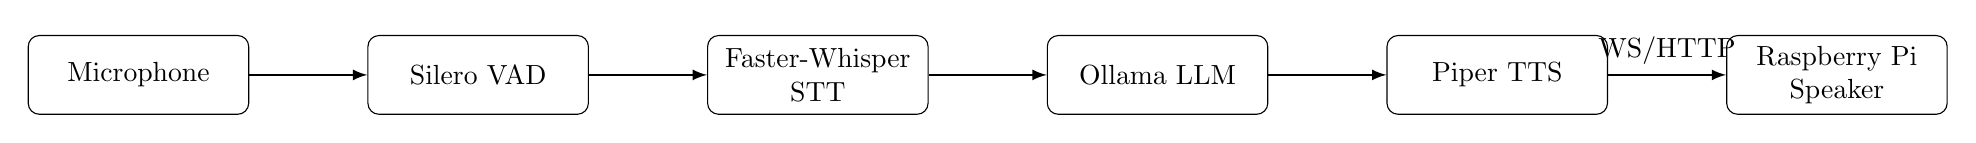
\begin{tikzpicture}[node distance=1.5cm, auto, >=latex]
    \tikzstyle{block}=[rectangle, draw, rounded corners, align=center, minimum width=2.8cm, minimum height=1cm]

    \node[block] (mic) {Microphone};
    \node[block, right=of mic] (vad) {Silero VAD};
    \node[block, right=of vad] (stt) {Faster-Whisper\\STT};
    \node[block, right=of stt] (llm) {Ollama LLM};
    \node[block, right=of llm] (tts) {Piper TTS};
    \node[block, right=of tts] (spk) {Raspberry Pi\\Speaker};

    \draw[->, thick] (mic) -- (vad);
    \draw[->, thick] (vad) -- (stt);
    \draw[->, thick] (stt) -- (llm);
    \draw[->, thick] (llm) -- (tts);
    \draw[->, thick] (tts) -- node[above] {WS/HTTP} (spk);
\end{tikzpicture}
\caption{End-to-end voice processing and playback pipeline.}
\end{figure}

\section{Sensor Integration}

\subsection{GPIO Architecture}
Sensor data is exposed through a Raspberry Pi endpoint and consumed by polling logic. This architecture decouples hardware sampling from assistant inference while preserving near-real-time control signals.

\subsection{Light Sensor Usage}
Light sensor values support optical educational interactions and can guide experiment-style responses or game state decisions.

\subsection{Button Input}
Button states can be used to trigger gameplay interactions, control state transitions, and provide direct tactile feedback in educational scenarios.

\subsection{Gyroscope Orientation Detection}
The orientation field is monitored continuously. Valid values are normalized and mapped to educational modes. This mapping drives spoken announcements and game-rule guidance.

\section{Orientation-Based Mode System}

\subsection{Mode Mapping}
\begin{longtable}{|>{\raggedright\arraybackslash}p{0.18\textwidth}|>{\raggedright\arraybackslash}p{0.32\textwidth}|>{\raggedright\arraybackslash}p{0.40\textwidth}|}
\hline
\textbf{Orientation} & \textbf{Mode} & \textbf{Behavior} \\
\hline
front & Logic Gate Level & Announces activation and then speaks Logic Gates rules. \\
\hline
right & Mirror Level & Announces activation and then speaks Reflection rules. \\
\hline
back & Silent & No TTS output. \\
\hline
left & Silent & No TTS output. \\
\hline
\end{longtable}

\subsection{Runtime Switching Logic}
When the detected orientation changes:
\begin{enumerate}
    \item Poll sensor endpoint and parse gyro orientation.
    \item Normalize orientation string.
    \item Lookup matching mode profile.
    \item Speak level announcement or game rules through TTS.
\end{enumerate}

The LLM prompt remains unchanged during face transitions so the assistant stays in a consistent STEM assistance mode.

\section{Game Integration}
The system is designed to interoperate with Unreal Engine educational mini-games. Sensor readings from buttons, light sensors, and orientation can be used as gameplay inputs, while the AI assistant provides contextual explanations or hints for each active level. Current mapping already aligns with game-oriented educational domains:
\begin{itemize}
    \item STEM tutoring on front orientation.
    \item Logical Systems Gateway challenge on left orientation.
    \item Optics and light-sensor experimentation on right orientation.
    \item Future expansion reserved for back orientation.
\end{itemize}

\section{Concurrency and System Reliability}

\subsection{Synchronization Improvements}
Two lock-based safeguards were introduced:
\begin{itemize}
    \item LLM request lock: protects prompt access and generation in concurrent runtime scenarios.
    \item TTS lock: prevents overlapping audio playback between face announcements/rules and assistant replies.
\end{itemize}

\subsection{Reliability Characteristics}
The gyro poller runs in a daemon thread and continues operation across transient endpoint failures, logging warnings and retrying based on configured polling intervals. This approach improves robustness for real-world sensor intermittency.

\section{Environment Configuration}
Configuration is loaded from environment variables via .env parsing in config.py. Key runtime parameters include:
\begin{itemize}
    \item Audio and VAD parameters: sample rate, chunk duration, speech thresholds.
    \item STT parameters: Whisper model, device, compute type.
    \item LLM parameters: Ollama URL, model, keep alive, timeout, base system prompt.
    \item Gyro parameters: URL, polling interval, request timeout.
    \item TTS and playback parameters: Piper binary/model/config, WebSocket and HTTP playback settings.
\end{itemize}

Important recently added keys:
\begin{itemize}
    \item VA\_GYRO\_URL
    \item VA\_GYRO\_POLL\_INTERVAL
    \item VA\_GYRO\_TIMEOUT
\end{itemize}

\section{Current Limitations}
\begin{itemize}
    \item Level 3 remains a placeholder mode and does not yet implement full educational logic.
    \item README baseline documentation does not yet include all orientation-mode implementation details.
    \item Orientation switching currently relies on immediate value changes and may benefit from debounce stability filtering.
\end{itemize}

\section{Future Improvements}
\begin{itemize}
    \item Move per-level prompt text into environment variables for no-code tuning.
    \item Add orientation debounce and temporal filtering to reduce accidental mode flips.
    \item Add startup health checks for sensor and playback endpoints.
    \item Add tests for orientation normalization, mapping, and spoken rules behavior.
    \item Add optional per-face debounce windows to reduce accidental rapid re-announcements.
\end{itemize}

\section{Conclusion}
The IA Companion demonstrates a practical embedded AI assistant architecture that combines local speech intelligence, local language generation, hardware sensor integration, and educational mode adaptation. The implemented orientation-driven announcement and rules system establishes a strong foundation for physically interactive learning experiences while preserving a stable STEM assistant behavior. With incremental reliability enhancements and expanded game content, the platform can evolve into a robust multi-domain educational companion suitable for classrooms, labs, and interactive demonstrations.

\section*{Appendix A: Representative Code Snippets}

\subsection*{A.1 Face-Driven Announcement Logic}
\begin{lstlisting}[style=pythonstyle]
LEVEL_BY_ORIENTATION = {
    "front": (
        "Logic gate level activated. "
        "Logic Gates: Press the buttons to send signals through the logic "
        "circuit. Your goal is to activate the final AND gate."
    ),
    "right": (
        "Mirror level activated. "
        "Reflection: Cover the light sensor to send a signal that rotates "
        "the mirrors. Adjust all three mirrors correctly to guide the light "
        "toward the prism and discover what happens when light passes "
        "through it."
    ),
    "back": "",
    "left": "",
}

if orientation and orientation != last_orientation:
    announcement = LEVEL_BY_ORIENTATION[orientation]
    if announcement.strip():
        with speak_lock:
            tts.speak(announcement)
\end{lstlisting}

\subsection*{A.2 Architecture Overview Diagram}
\begin{figure}[H]
\centering
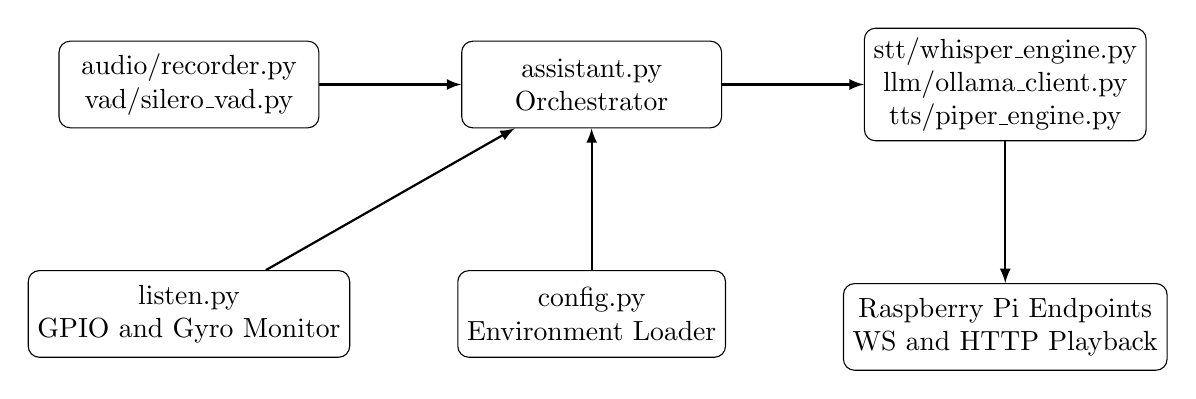
\begin{tikzpicture}[node distance=1.8cm, auto, >=latex]
    \tikzstyle{box}=[rectangle, draw, rounded corners, align=center, minimum width=3.3cm, minimum height=1.1cm]

    \node[box] (assist) {assistant.py\\Orchestrator};
    \node[box, left=of assist] (audio) {audio/recorder.py\\vad/silero\_vad.py};
    \node[box, right=of assist] (infer) {stt/whisper\_engine.py\\llm/ollama\_client.py\\tts/piper\_engine.py};
    \node[box, below=of assist] (cfg) {config.py\\Environment Loader};
    \node[box, below=of audio] (sensor) {listen.py\\GPIO and Gyro Monitor};
    \node[box, below=of infer] (pi) {Raspberry Pi Endpoints\\WS and HTTP Playback};

    \draw[->, thick] (audio) -- (assist);
    \draw[->, thick] (assist) -- (infer);
    \draw[->, thick] (cfg) -- (assist);
    \draw[->, thick] (sensor) -- (assist);
    \draw[->, thick] (infer) -- (pi);
\end{tikzpicture}
\caption{Software architecture relationships across orchestrator, inference modules, configuration, and Raspberry Pi interfaces.}
\end{figure}

\end{document}
